\subsection{Slave Aktuator Design}
\label{ch:slave_aktuator_design}

På Figur \ref{fig:stm_psoc_aktuator} vises virkemåden for SW på PSoC 4 i blokken Slave Aktuator. 
Grundprincippet er, at slaven hele tiden er klar til at modtage data på \IIC bussen, da dette sker vha. et interrupt. 
Når den ikke er i gang med at modtage data, opdaterer den et status register - hvis der er modtaget data - og sammenligner det med et positionsregister. 
Hvis de to registre ikke er ens, indstiller den respektive porte for de forskellige aktuatorer og opdaterer positionsregistret. 

\begin{figure}[h]
\centering 
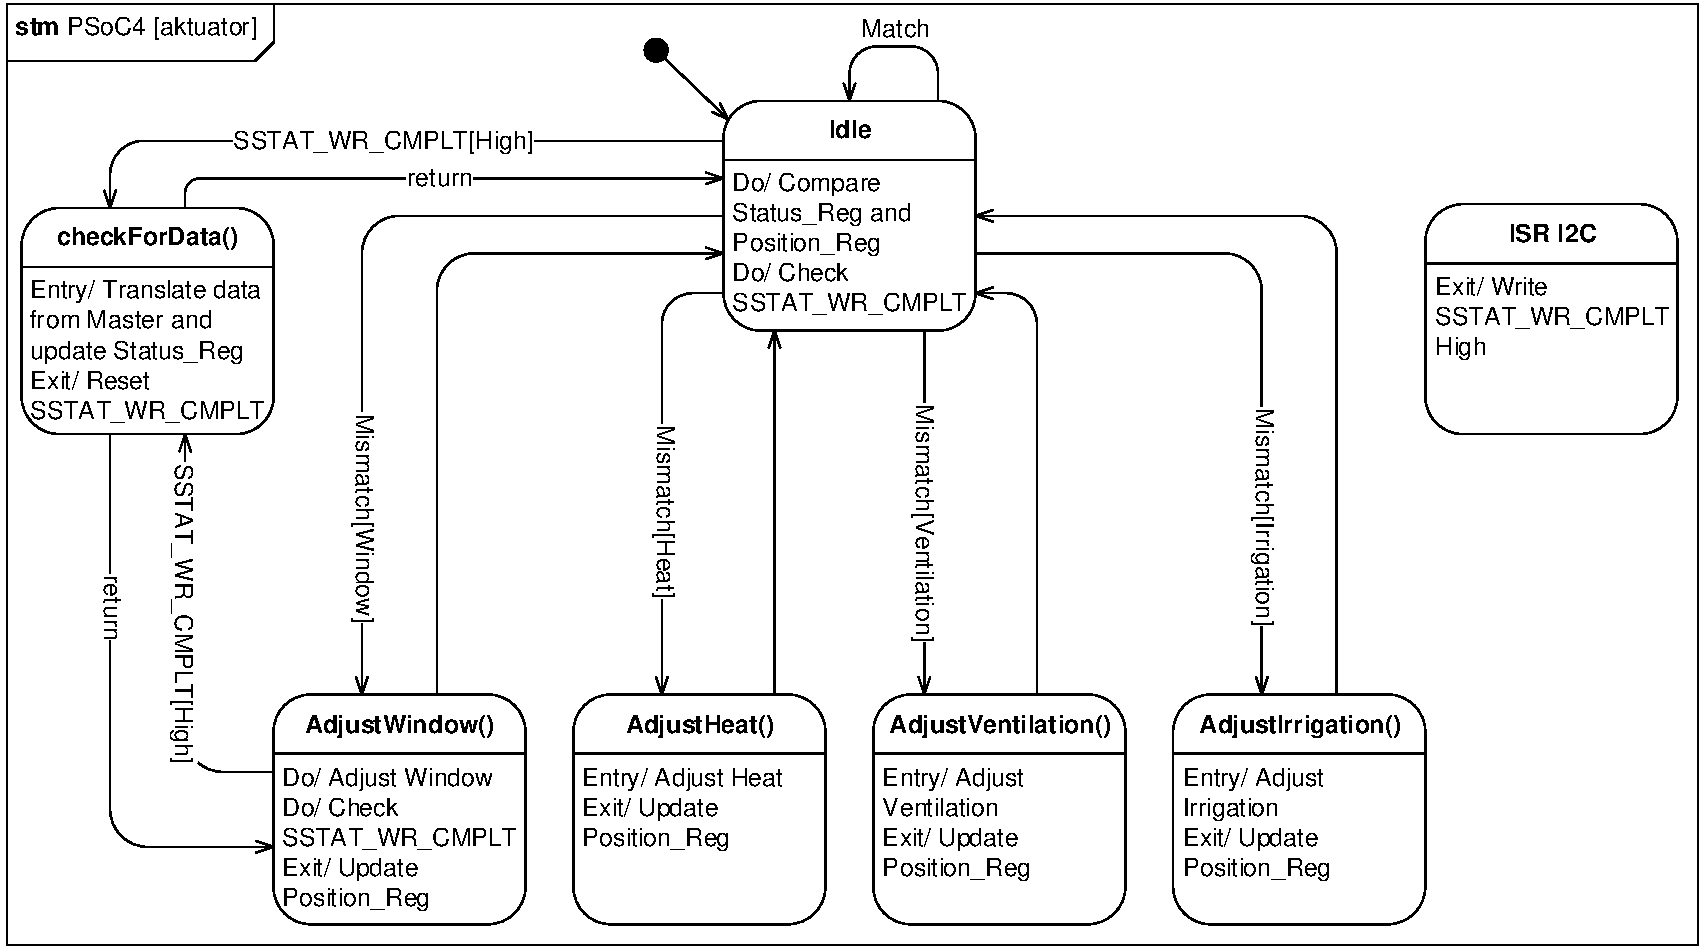
\includegraphics[width={\textwidth}, trim=0 0 0 0, clip=true] {../fig/stm_psoc_aktuator.pdf}
\caption{State Machine for software på underblokken PSoC 4 i Aktuator}
\label{fig:stm_psoc_aktuator}
\end{figure}

De seks porte, som styrer vanding ved tilhørende jordfugtsensorer, er ikke koblet til noget, de giver blot mulighed for at tilkoble et vandingssystem til AutoGreen.

Portene til styring af varmelegeme, ventilatorer og steppermotor er koblet sammen med tre forskellige Mosfetdrivere. 
De tre drivere er grundlæggende ens designet; på næste side er designet for steppermotoren vist. 

\clearpage

\begin{figure}[h]
\centering 
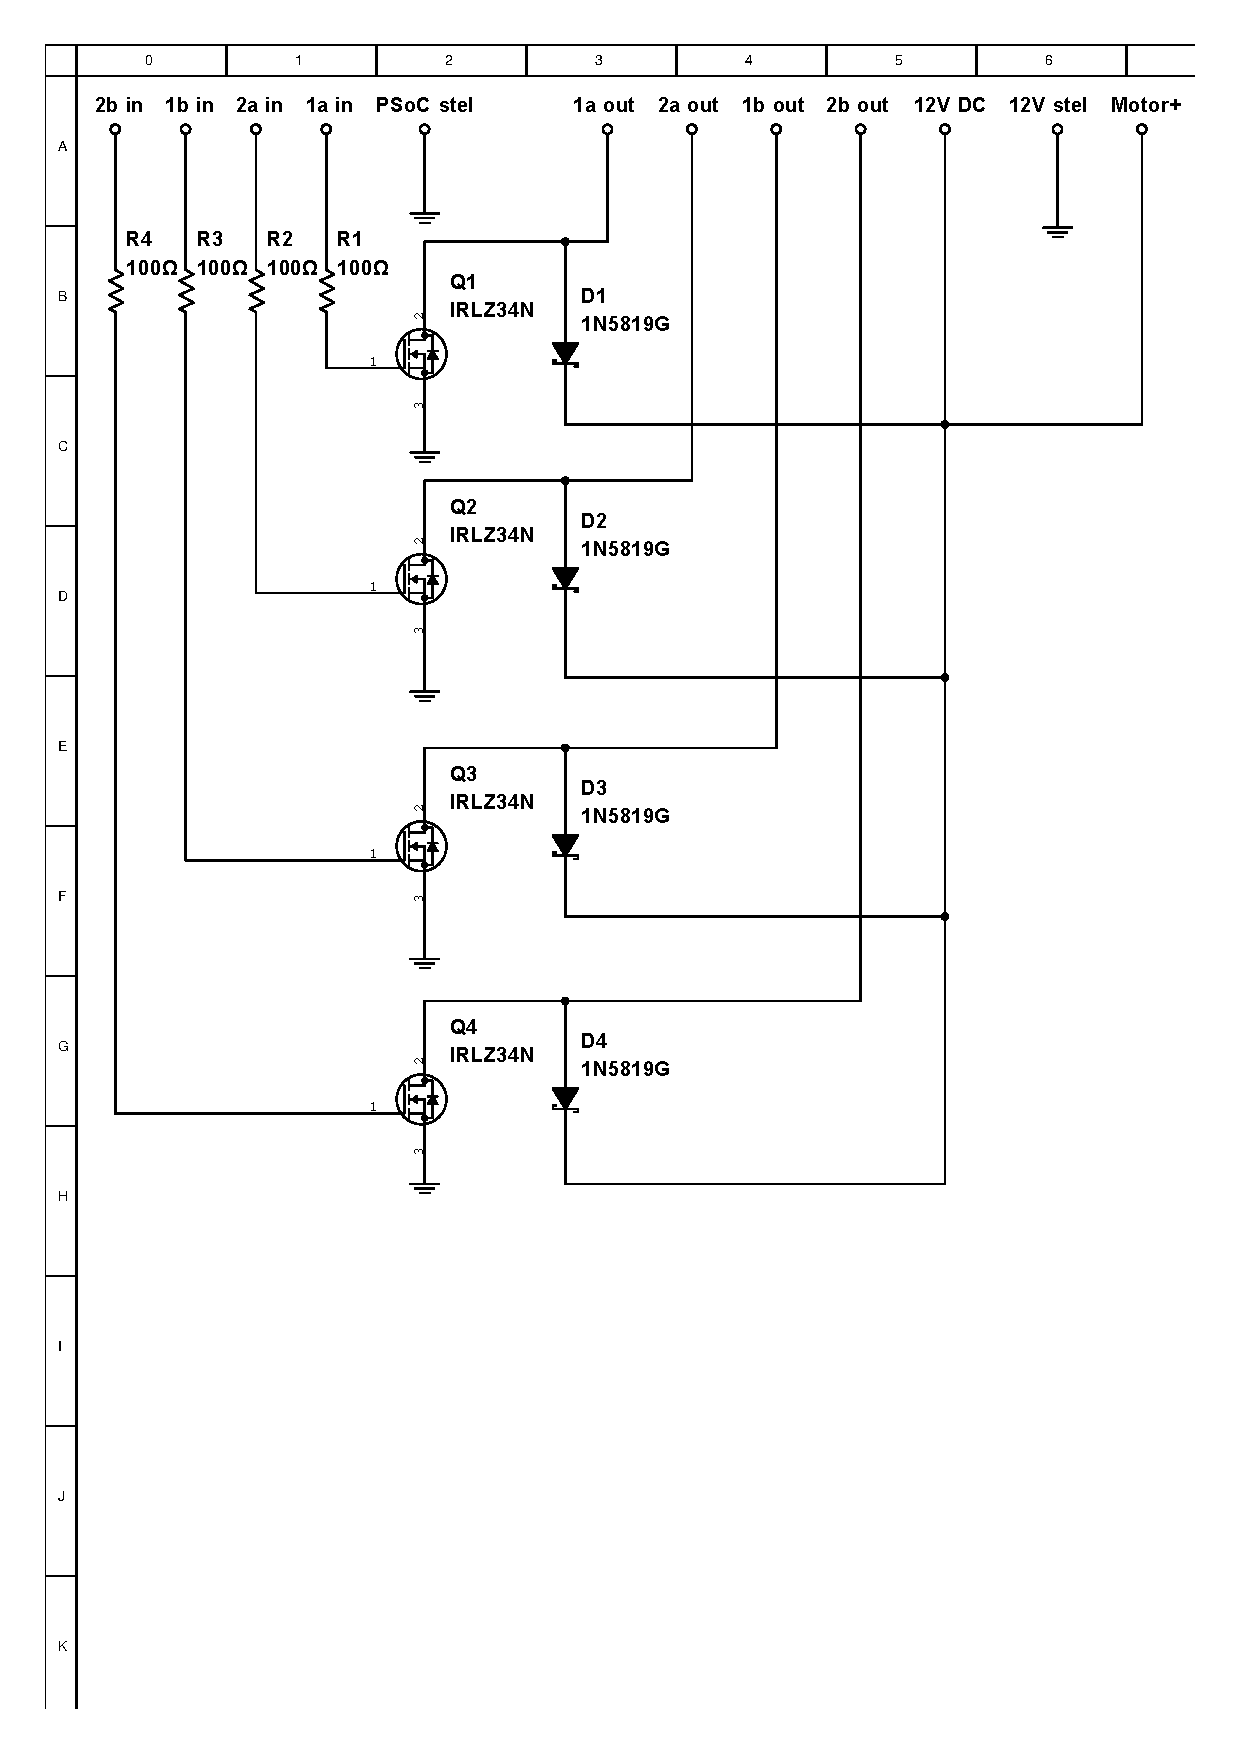
\includegraphics[width={\textwidth-1cm}, trim= 40 260 0 40, clip=true] {../fig/multisim_vinduesmotor_mosfetdriver.pdf}
\caption{Kredsløb for Mosfet Driver i underblokken Vinduesmotor}
\label{fig:multisim_vinduesmotor_mosfetdriver}
\end{figure}

Mosfetdriveren på Figur \ref{fig:multisim_vinduesmotor_mosfetdriver} indeholder fire mosfet transistorer, da de fire indgange på motoren ikke skal åbne og lukke samtidigt. 
Motoren får hele tiden 12V DC, og transistorerne åbner og lukker for stel.
De fire dioder er beskyttelsesdioder, som sikrer mod spændingspeak fra spolerne i motoren, når de afbrydes. 
De fire modstande er også beskyttelse af PSoC'en; såfremt mosfet'erne fejler, vil der afsættes effekt i modstandene frem for i PSoC'en.

For den fulde beskrivelse, se afsnit \ref{P-sec:Aktuator_Design} \nameref{P-sec:Aktuator_Design} på side \pageref{P-sec:Aktuator_Design} i projektdokumentationen.

\mbox{}

Som udgangspunkt var tanken at gøre designet fuldstændigt interruptbaseret for at effektivisere afvikling af koden.
Dette voldte dog en del problemer under implementeringen, derfor blev designet som beskrevet ovenfor. 

Der blev desuden eksperimenteret med brug af PSoC'ens flash hukommelse, så aktuel status på aktuatorer ikke gik tabt ved strømafbrydelse. 
Dette voldte desværre også problemer, hvorfor dette ikke er en del af designet.


\clearpage